\chapter{Implementacija i korisničko sučelje}
		
		
		\section{Korištene tehnologije i alati}
			
			
			Komunikacija u timu realizirana je korištenjem aplikacije WhatsApp\footnote{\url{https://www.whatsapp.com/}}, a organizacija i podjela zadataka korištenjem aplikacije Trello\footnote{\url{https://trello.com/}}. 
			Za izradu UML dijagrama korišten je alat Astah UML\footnote{\url{https://astah.net/products/astah-uml/}}, a kao sustav za upravljanje
			izvornim kodom Git\footnote{\url{https://git-scm.com/}}. Udaljeni repozitorij projekta dostupan je na web platformi
			GitLab\footnote{\url{https://gitlab.com/}}.
			
			Kao razvojno okruženje korišten je Microsoft Visual Studio Code\footnote{\url{https://code.visualstudio.com/}} - 
			besplatni uređivač teksta tvrtke Microsoft. Sadrži podršku za debugging, izvođenje zadataka te sustav za upravljanje izvornim kodom. Koristi se za razvoj računalnih
			programa za operacijski sustav Windows, kao i za web-stranice, web-aplikacije,
			te ostale web-usluge. Jedan je od najpopularnijih razvojnih alata. Bazira se na radnom sučelju Electron, koje se koristi za razvoj Node.js Web aplikacija.
			
			
			Aplikacija je napisana koristeći radni okvir Django\footnote{\url{https://www.djangoproject.com/}} i jezik Python\footnote{\url{https://www.python.org/}} za
			izradu backenda te Nuxt.js\footnote{\url{https://nuxtjs.org/}} i jezik JavaScript\footnote{\url{https://www.javascript.com/}} za izradu frontenda. Nuxt.js je radni okvir koji se bazira na Vue.js\footnote{\url{https://vuejs.org/}}, Node.js\footnote{\url{https://nodejs.org/en/}}, Webpack\footnote{\url{https://webpack.js.org/}} i Babel.js\footnote{\url{https://babeljs.io/}}. Podržava generiranje statičkih web stranica i bazira se na modularnoj arhitekturi. Postoji preko 50 modula koji razvoj čine bržim i jednostavnijim. Django radni okvir omogućava brz razvoj sigurnih i održivih web stranica. Prati MTV (model-template-view) arhitekturni obrazac. Neke od poznatih stranica koje koriste Django su Instagram, Mozilla, The Washington Times, Bitbucket itd.
			
			Za lokalno upravljanje i slanje upita na bazu podataka koristili smo alat pgAdmin\footnote{\url{https://www.pgadmin.org/}}. Baza podataka se trenutno nalazi na poslužitelju Heroku\footnote{\url{https://www.heroku.com/}}.
			
			
			
			
			\eject 
		
	
		\section{Ispitivanje programskog rješenja}
			
			\textbf{\textit{dio 2. revizije}}\\
			
			 \textit{U ovom poglavlju je potrebno opisati provedbu ispitivanja implementiranih funkcionalnosti na razini komponenti i na razini cijelog sustava s prikazom odabranih ispitnih slučajeva. Studenti trebaju ispitati temeljnu funkcionalnost i rubne uvjete.}
	
			
			\subsection{Ispitivanje komponenti}
			U ovom ćemo poglavlju predstaviti 9 ispitnih slučajeva (unit testova). Svi se ispitni primjeri mogu pronaći u datoteci janezi/izvorniKod/backend/common/tests.py koja je sastavljena od 4 klase koje ukupno sadrže 9 testova te sadrži 137 linija programskog koda.
			
			\vspace{5mm} %5mm vertical space
			
			Ispitni slučajevi 1 i 2 odnose se na prijavu korisnika. Oba se ispitna slučaja nalaze u klasi AccountTests. U prvom se slučaju korisnik ne može prijaviti jer mu korisnički račun nije potvrđen, dok se u drugom slučaju, odmah nakon potvrde računa, korisnik može uspješno prijaviti. U prvom je slučaju očekivan odgovor 400 (pogreška), dok je u drugom slučaju očekivan odgovor 200. Oba ispitna primjera daju očekivani rezultat.
			
			\begin{figure}[H]
				\centering
				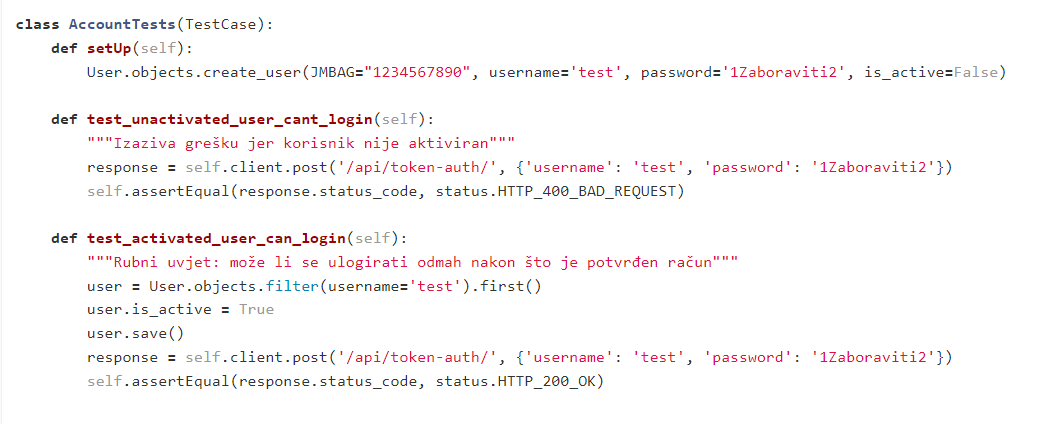
\includegraphics[scale=0.65]{slike/AccountTests.PNG}
				\caption{Ispitni slučajevi vezani za prijavu korisnika}
				\label{fig:promjene}
			\end{figure}
		
			Ispitni slučajevi 3 i 4 vezani su za administratora te provjeravaju ispravnost funkcionalnosti blokiranja korisnika. Oba se ispitna slučaja nalaze u klasi AdminTests. Prvi slučaj izaziva pogrešku (kod 401 UNAUTHORIZED) jer korisnik koji nije administrator pokušava blokirati račun drugog korisnika. U drugom slučaju, korisnik koji je administrator blokira korisnika i provjerava se točnost akcije. Oba ispitna primjera daju očekivani rezultat.
			
			\begin{figure}[H]
				\centering
				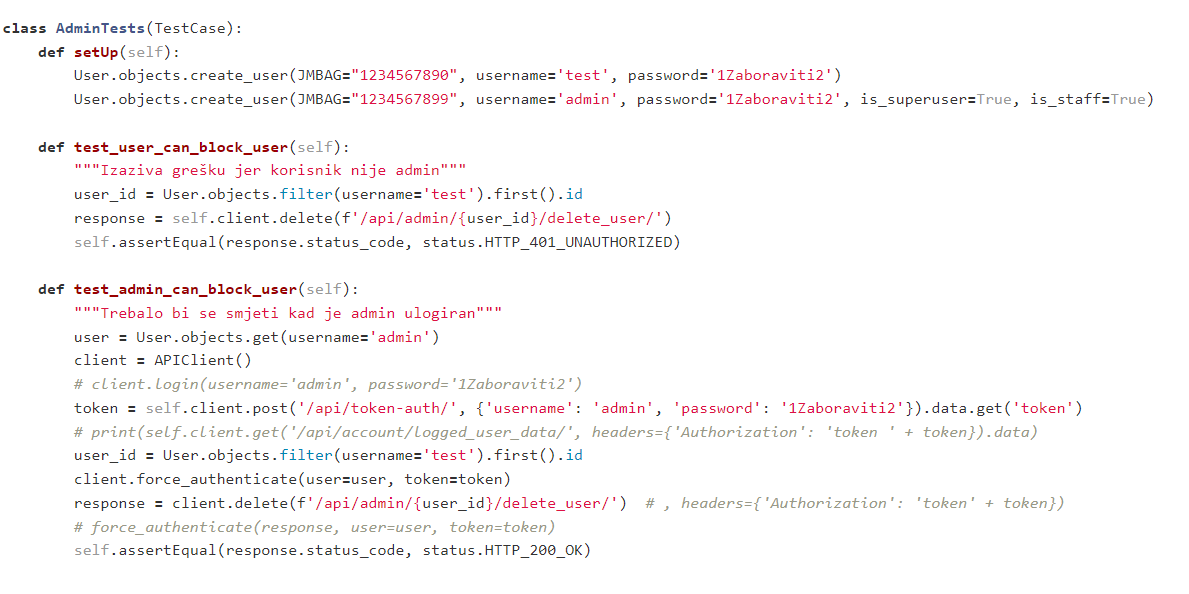
\includegraphics[scale=0.65]{slike/AdminTests.PNG}
				\caption{Ispitni slučajevi vezani za prijavu korisnika}
				\label{fig:promjene}
			\end{figure}
	
			Ispitni slučajevi 5, 6 i 7 odnose se na funkcionalnost vraćanja košare. Oba se ispitna slučaja nalaze u klasi WorkerTests. Prvi slučaj predstavlja situaciju u kojoj korisnik koji ne radi u praonici pokušava vratiti košaru. Taj bi slučaj trebao vratiti poruku 401 UNAUTHORIZED kako netko ne bi mogao zloupotrebljavati povrat košare. Drugi test provjerava ponašanje aplikacije u slučaju kad radnik pokuša označiti da je netko vratio košaru te osim provjere uspješnosti (kod 200), provjerava se i je li se broj košara tog korisnika smanjio na 0 (linija 75 u kodu). Sva tri ispitna primjera daju rezultat u skladu s očekivanjima.
			
			\begin{figure}[H]
				\centering
				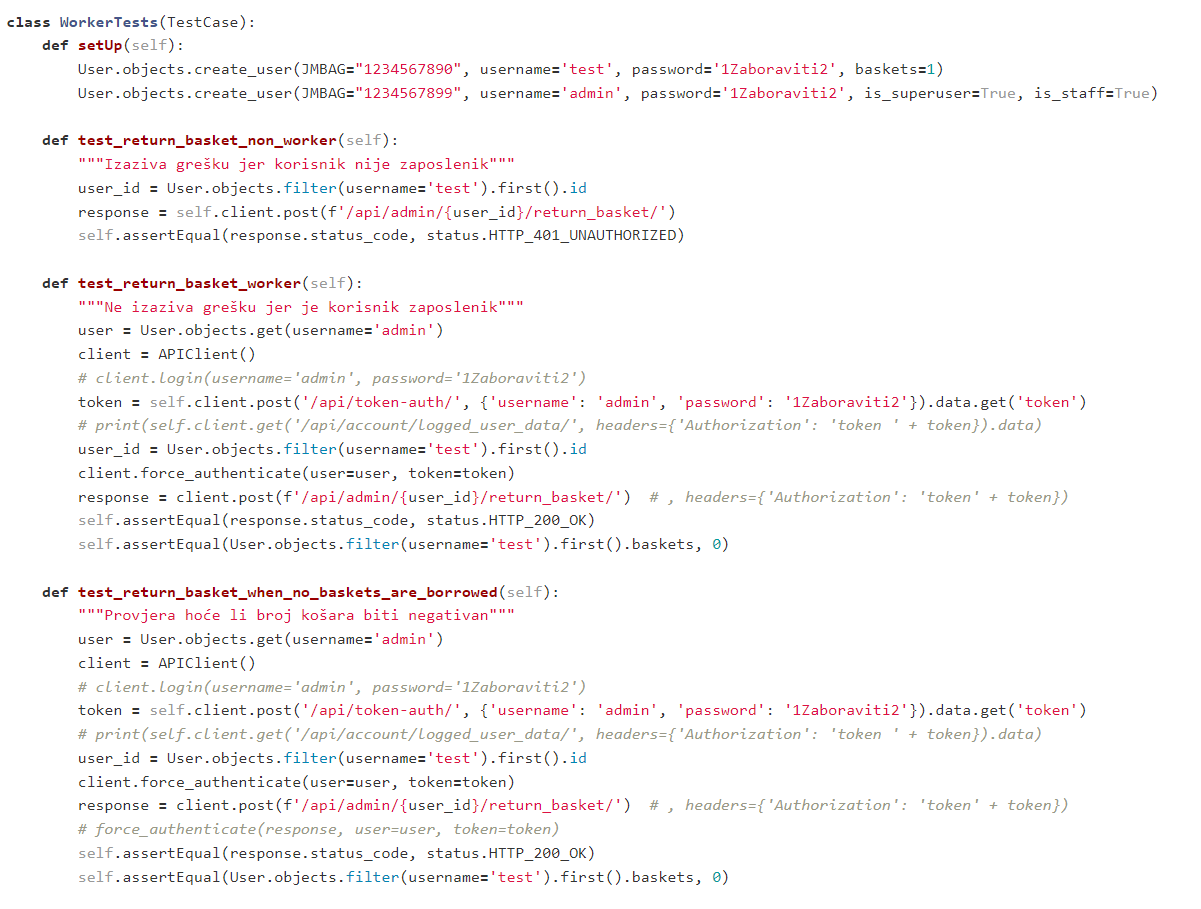
\includegraphics[scale=0.65]{slike/WorkerTests.PNG}
				\caption{Ispitni slučajevi vezani za vraćanje košara}
				\label{fig:promjene}
			\end{figure}
		
			Posljednja klasa ispitnih primjera, nalazi se u klasi AppointmentTests i sadrži ispitne primjere 8 i 9. Osmi ispitni primjer provjerava može li neregistrirani korisnik napraviti rezervaciju te je očekivano ponašanje pogreška s kodom 401. Ispitni primjer br. 9 ispituje rezervaciju termina nakon prijave i provjerava je li radnja bila uspješna (kod 201 CREATED). Oba ispitna primjera daju očekivani rezultat.
			
			\begin{figure}[H]
				\centering
				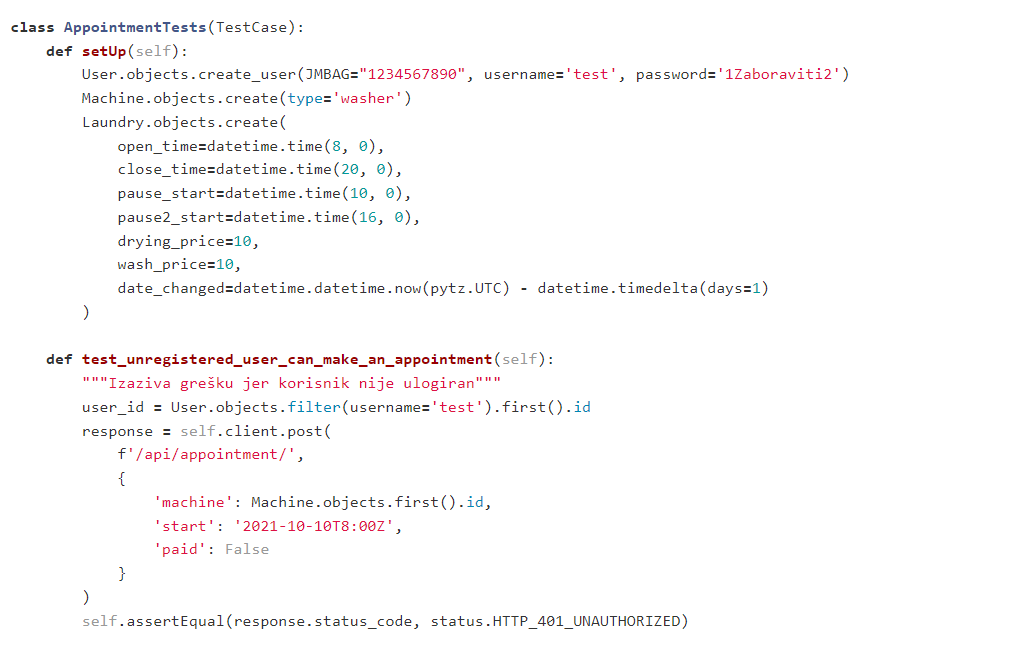
\includegraphics[scale=0.65]{slike/AppointmentTests1.PNG}
				\caption{Ispitni slučajevi vezani za rezervaciju termina, slika 1/2}
				\label{fig:promjene}
			\end{figure}
		
			\begin{figure}[H]
				\centering
				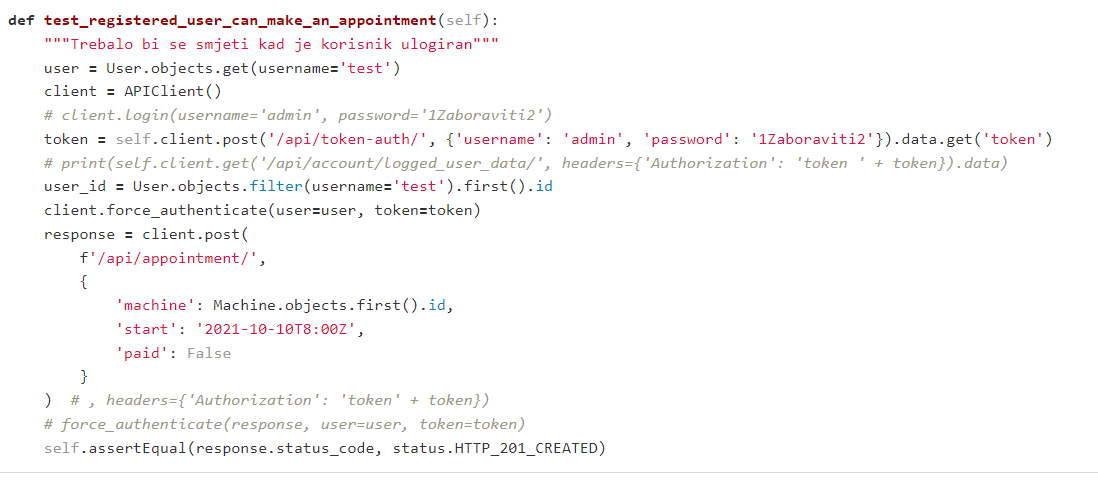
\includegraphics[scale=0.65]{slike/AppointmentTests2.PNG}
				\caption{Ispitni slučajevi vezani za rezervaciju termina, slika 2/2}
				\label{fig:promjene}
			\end{figure}
		
			Svi se spomenuti testovi mogu pokrenuti iz terminala aktivacijom virtualnog okruženja, pozicioniranjem u mapu backend i pozivanjem naredbe ./manage.py test. Kao što je već spomenuto, svi se testovi izvršavaju točno, a slika ~\ref{fig:TestsTerminal} pokretanja naredbe ./manage.py test dana je u prilogu. 
			
			\begin{figure}[H]
				\centering
				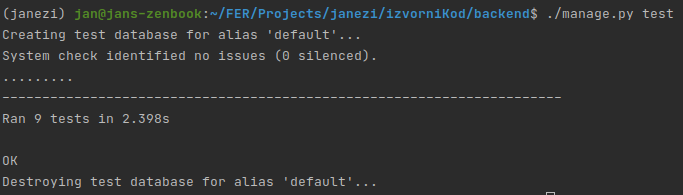
\includegraphics[scale=0.65]{slike/TestsTerminal.PNG}
				\caption{Pokretanje svih ispitnih slučajeva u terminalu}
				\label{fig:TestsTerminal}
			\end{figure}
			
			
			\subsection{Ispitivanje sustava}
			
			 \textit{Potrebno je provesti i opisati ispitivanje sustava koristeći radni okvir Selenium\footnote{\url{https://www.seleniumhq.org/}}. Razraditi \textbf{minimalno 4 ispitna slučaja} u kojima će se ispitati redovni slučajevi, rubni uvjeti te poziv funkcionalnosti koja nije implementirana/izaziva pogrešku kako bi se vidjelo na koji način sustav reagira kada nešto nije u potpunosti ostvareno. Ispitni slučaj se treba sastojati od ulaza (npr. korisničko ime i lozinka), očekivanog izlaza ili rezultata, koraka ispitivanja i dobivenog izlaza ili rezultata.\\ }
			 
			 \textit{Izradu ispitnih slučajeva pomoću radnog okvira Selenium moguće je provesti pomoću jednog od sljedeća dva alata:}
			 \begin{itemize}
			 	\item \textit{dodatak za preglednik \textbf{Selenium IDE} - snimanje korisnikovih akcija radi automatskog ponavljanja ispita	}
			 	\item \textit{\textbf{Selenium WebDriver} - podrška za pisanje ispita u jezicima Java, C\#, PHP koristeći posebno programsko sučelje.}
			 \end{itemize}
		 	\textit{Detalji o korištenju alata Selenium bit će prikazani na posebnom predavanju tijekom semestra.}
			
			\eject 
		
		
		\section{Dijagram razmještaja}
			Na poslužiteljskom računalu se nalaze web poslužitelj i poslužitelj baze podataka. Oni se nalaze unutar Heroku izvršne okoline koja sadrži usluge koje organiziraju i upravljaju izvršavanjem i razmjerom aplikacije. Frontend i backend se pokreću u Dynosima. To su lagana, izolirana okruženja koja pružaju računalnu snagu, memoriju, OS i "Ephemeral" datotečni sustav. Klijenti koriste web preglednik kako bi pristupili web aplikaciji.  Sustav je baziran na arhitekturi ”klijent-poslužitelj”, a komunikacija između računala korisnika (klijent, zaposlenik, administrator) i poslužitelja odvija se preko HTTPS veze.
			
			\begin{figure}[H]
				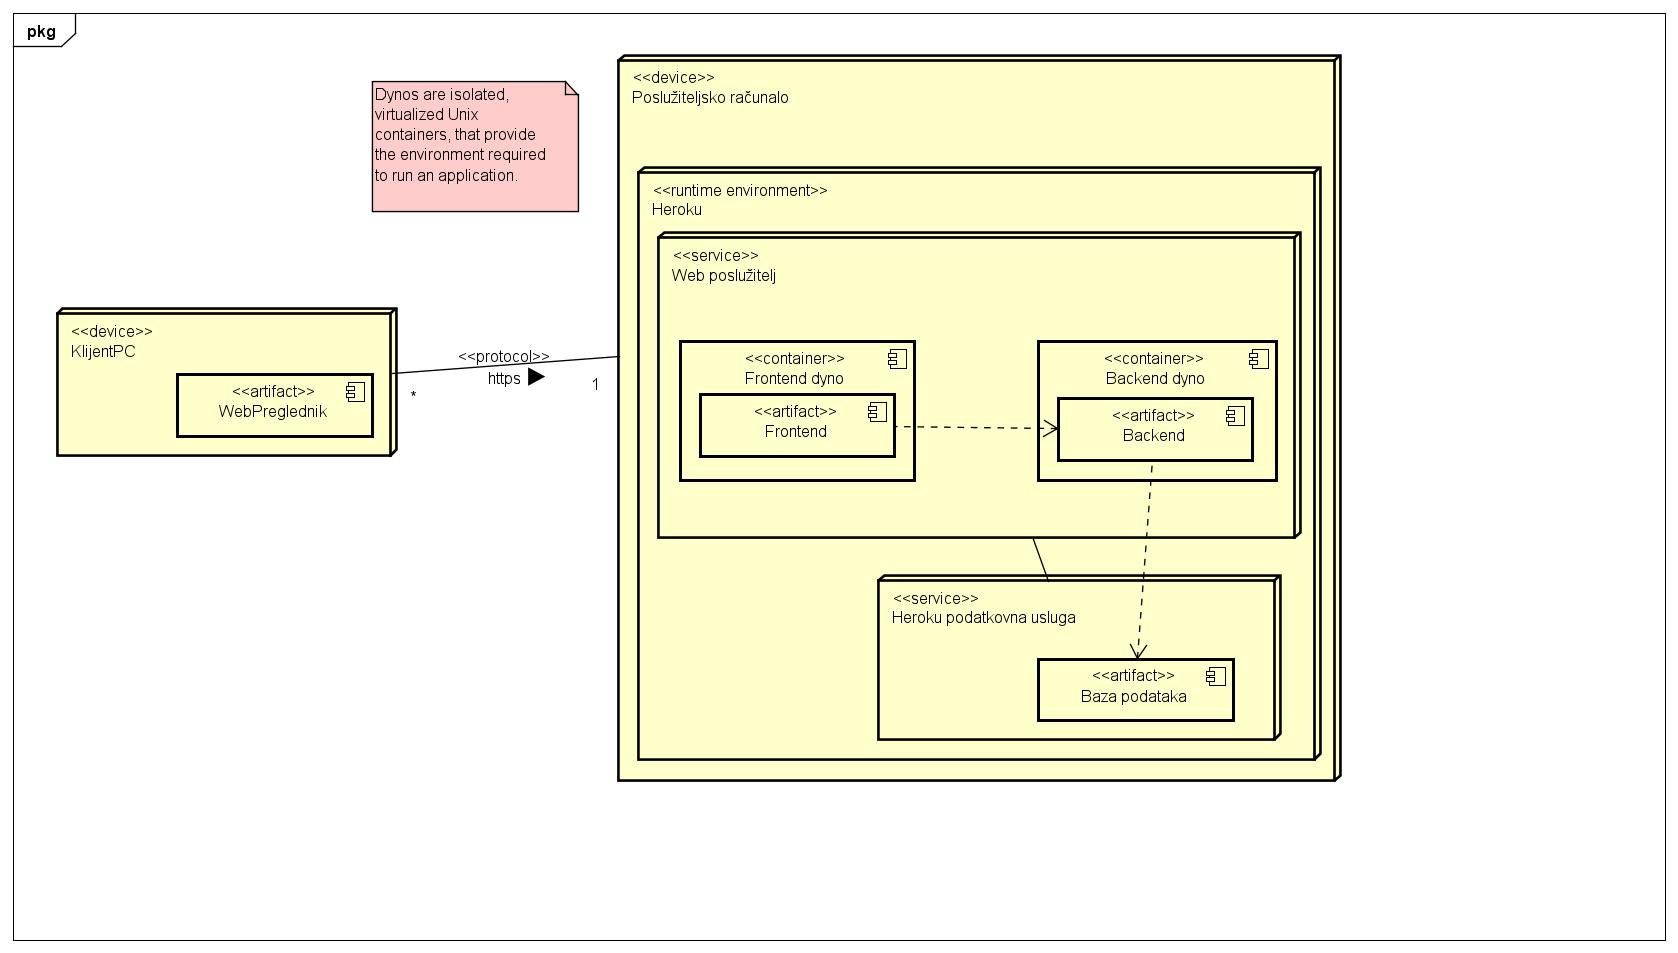
\includegraphics[width=1\linewidth]{slike/dijagram-razmjestaja.jpg}
				\centering
				\caption{Dijagram stanja}
				\label{fig:dijagram_razmjestaja}
			\end{figure}
			\eject 
		
		\section{Upute za puštanje u pogon}
		
			Za puštanje u pogon, koristili smo heroku server (https://www.heroku.com/). Prvi korak za puštanje u pogon bila je podjela aplikacije na poslužiteljsku i korisničku stranu. Svaki se od tih djelova aplikacije treba staviti u zasebnu mapu. Imena mapi moraju odgovarati imenima aplikacija na heroku poslužitelju. Mi smo se odlučili za naziv terminko za korisničku stranu te naziv terminko1 za poslužiteljsku stranu.
			
			\begin{figure}[H]
				\centering
				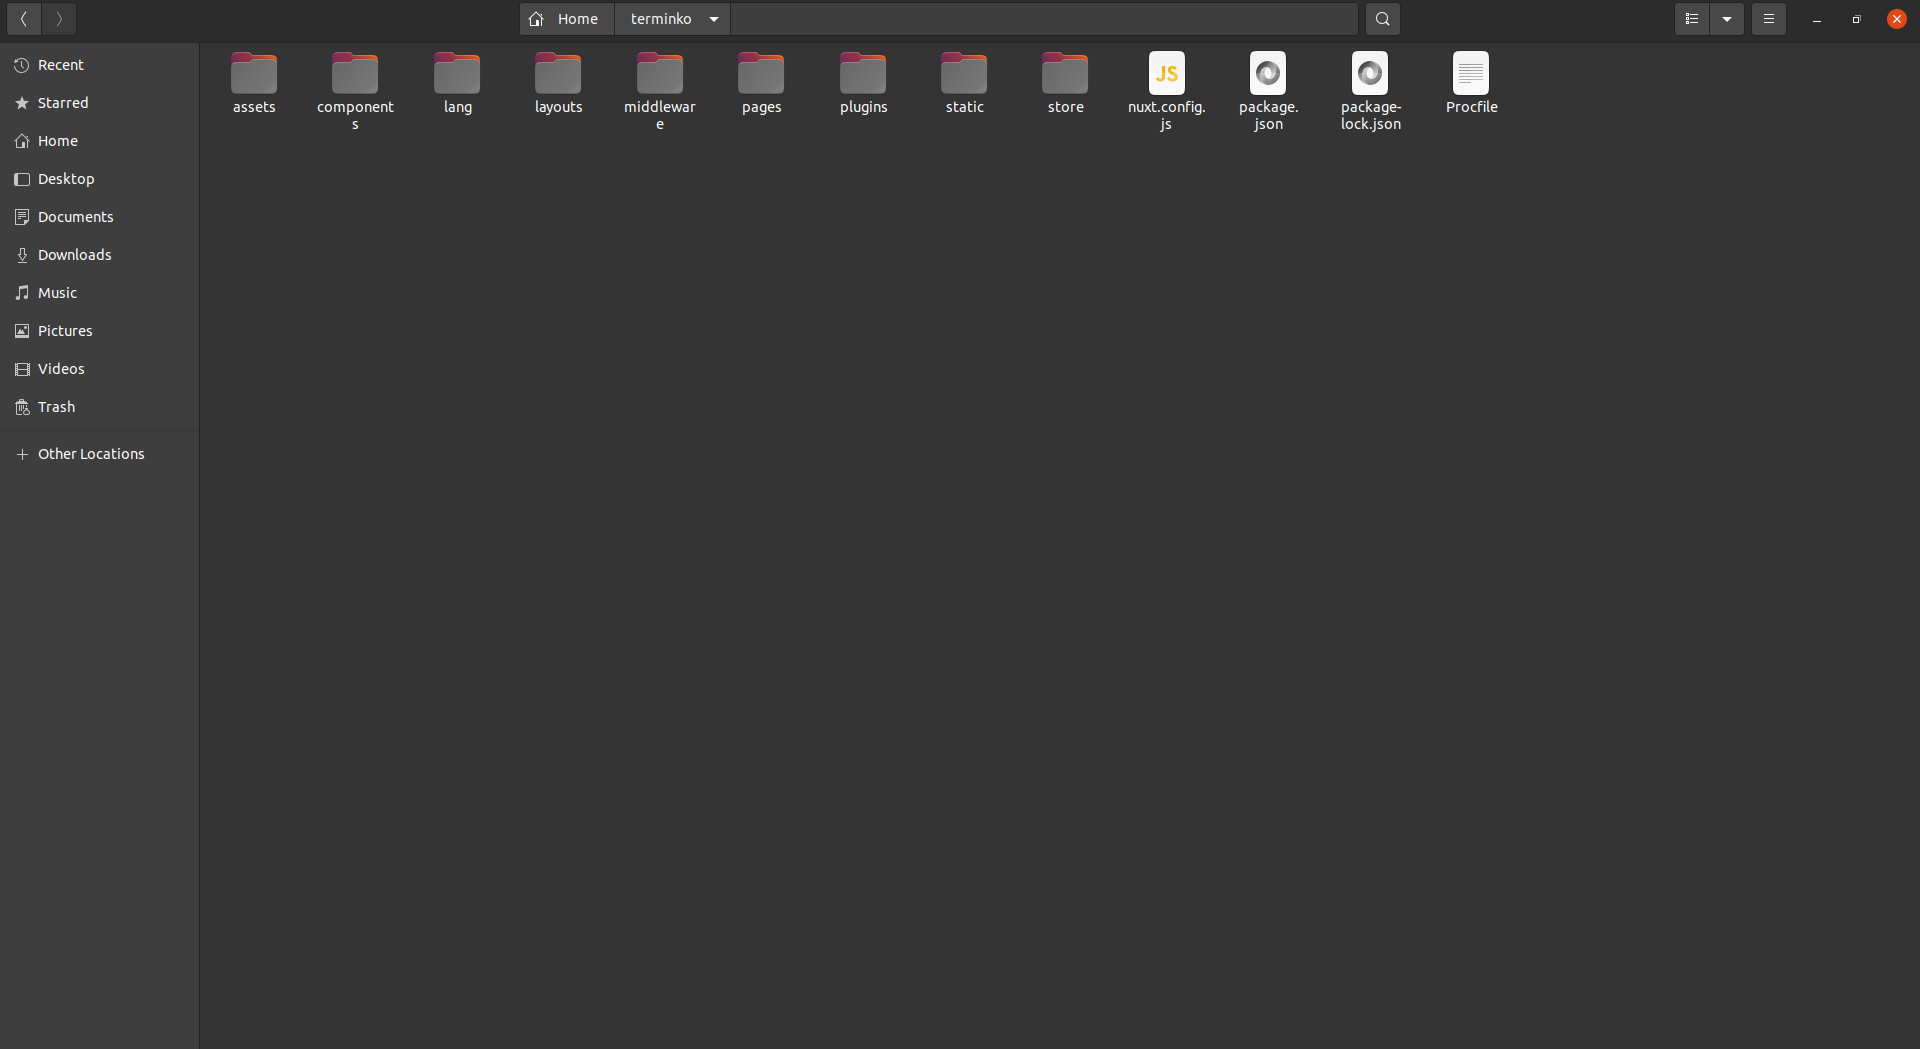
\includegraphics[scale=0.25]{slike/FrontendMapa.PNG}
				\caption{Mapa za frontend: terminko}
				\label{fig:promjene}
			\end{figure}
			
			\begin{figure}[H]
				\centering
				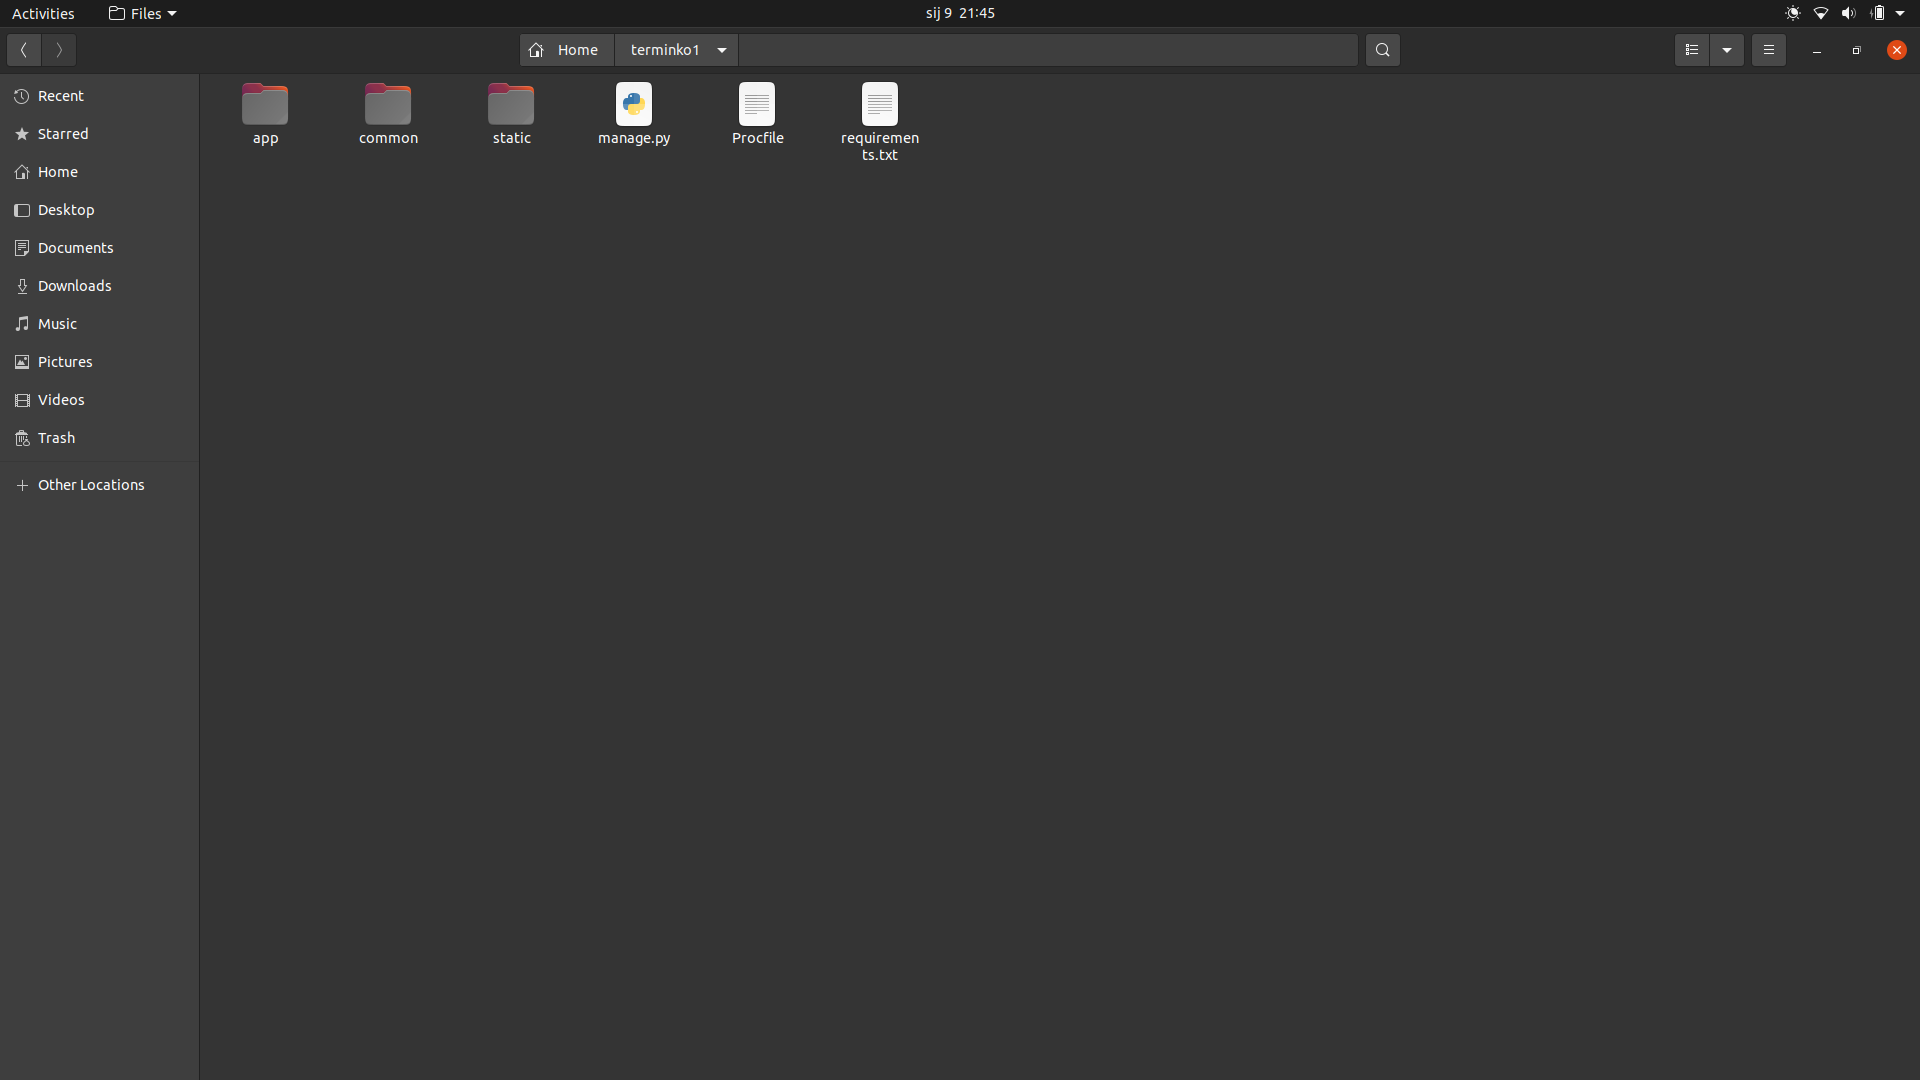
\includegraphics[scale=0.25]{slike/BackendMapa.PNG}
				\caption{Mapa za backend: terminko1}
				\label{fig:promjene}
			\end{figure}
		
			Prvo smo na heroku postavili klijentsku stranu na način da smo prvo napravili aplikaciju terminko. Nakon izrade aplikacije, u odjeljku settings postavili smo konfiguracijske varijable kako je prikazano na slici te smo dodali "buildpack" za Node.js.
			
			\begin{figure}[H]
				\centering
				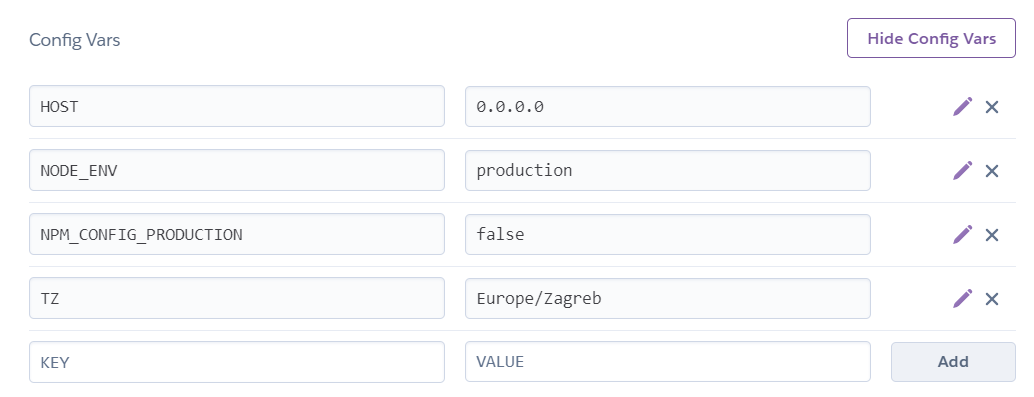
\includegraphics[scale=0.65]{slike/KonfiguracijaFrontend.PNG}
				\caption{Konfiguracija za frontend}
				\label{fig:promjene}
			\end{figure}
		
			\begin{figure}[H]
				\centering
				\includegraphics[scale=0.45]{slike/BuildpackFrontend.PNG}
				\caption{Buildpack za frontend}
				\label{fig:promjene}
			\end{figure}
		
			Na lokalnom smo stroju, u mapu terminko dodali Procfile i u nuxt-config.js dodali novi base-URL za upite na backend
			
			\begin{figure}[H]
				\centering
				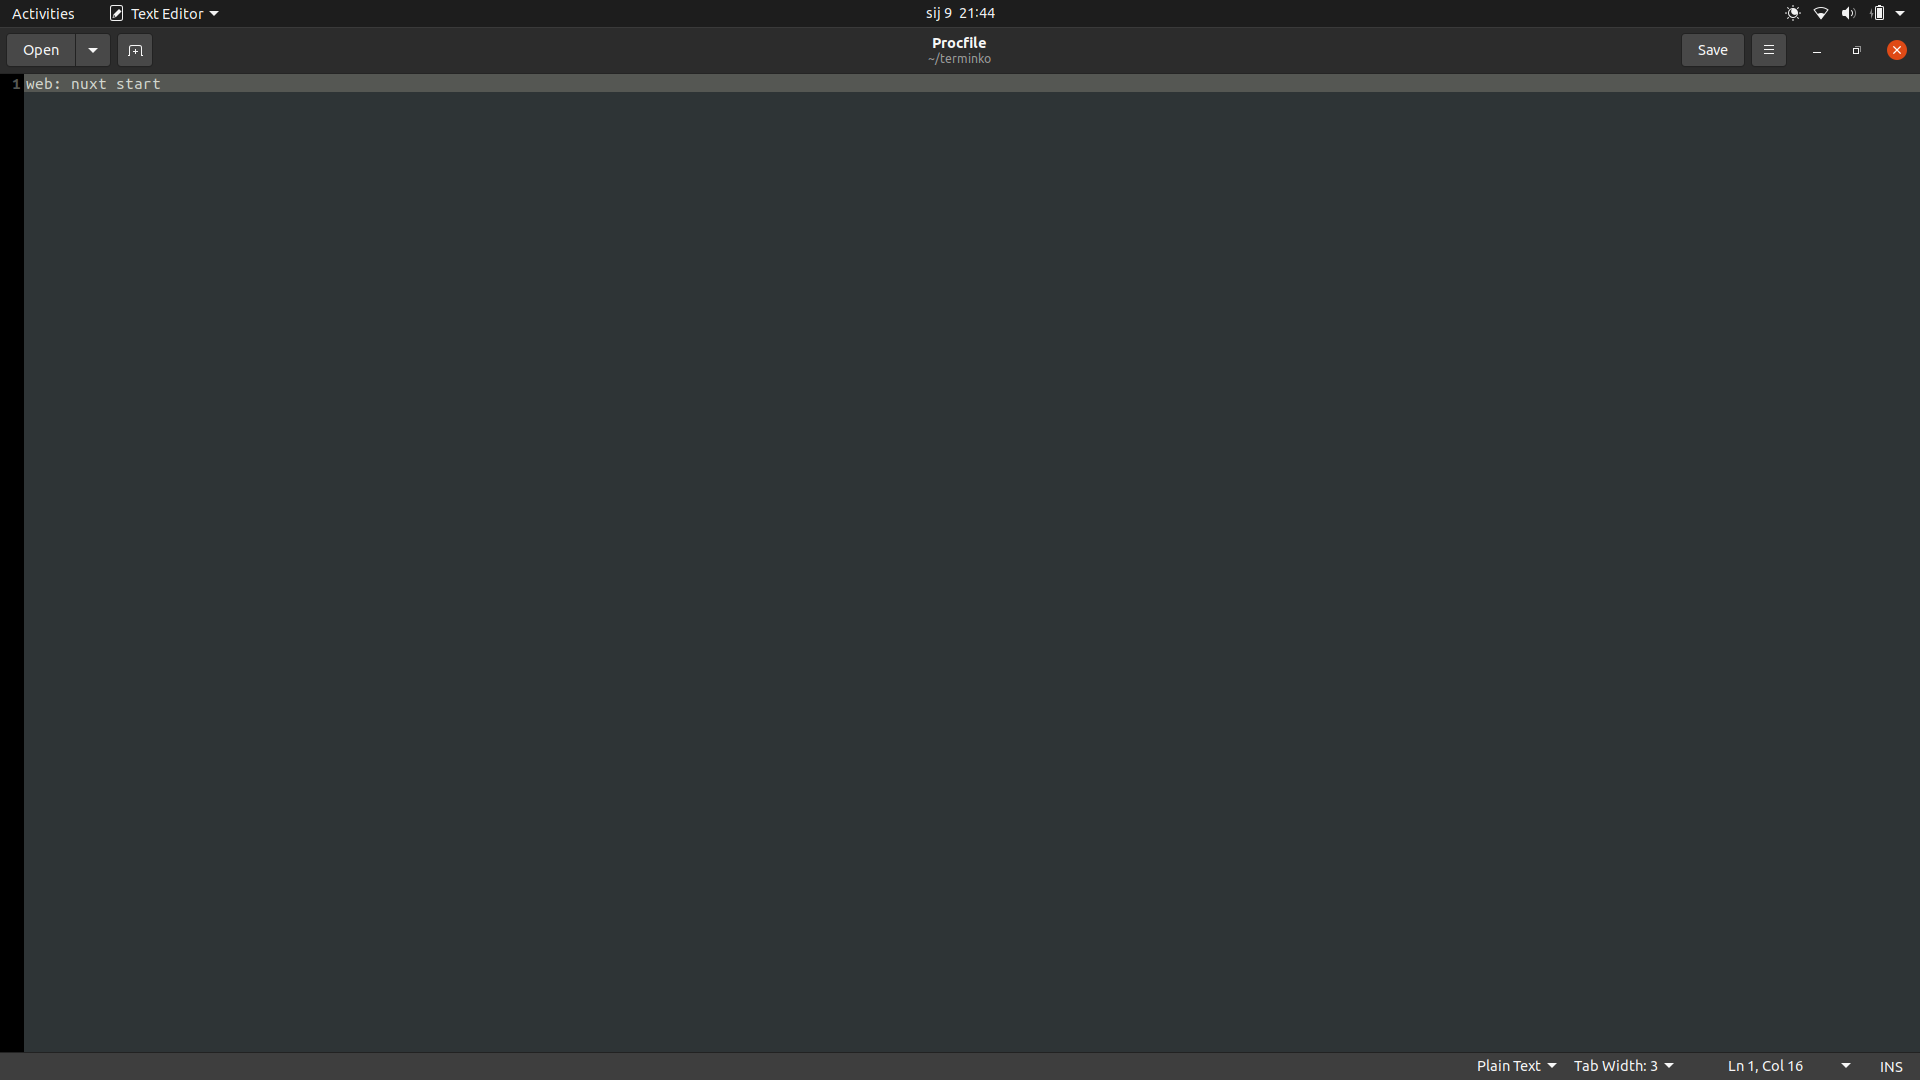
\includegraphics[scale=0.25]{slike/ProcFileFrontend.PNG}
				\caption{Procfile za frontend}
				\label{fig:promjene}
			\end{figure}
			
			\begin{figure}[H]
				\centering
				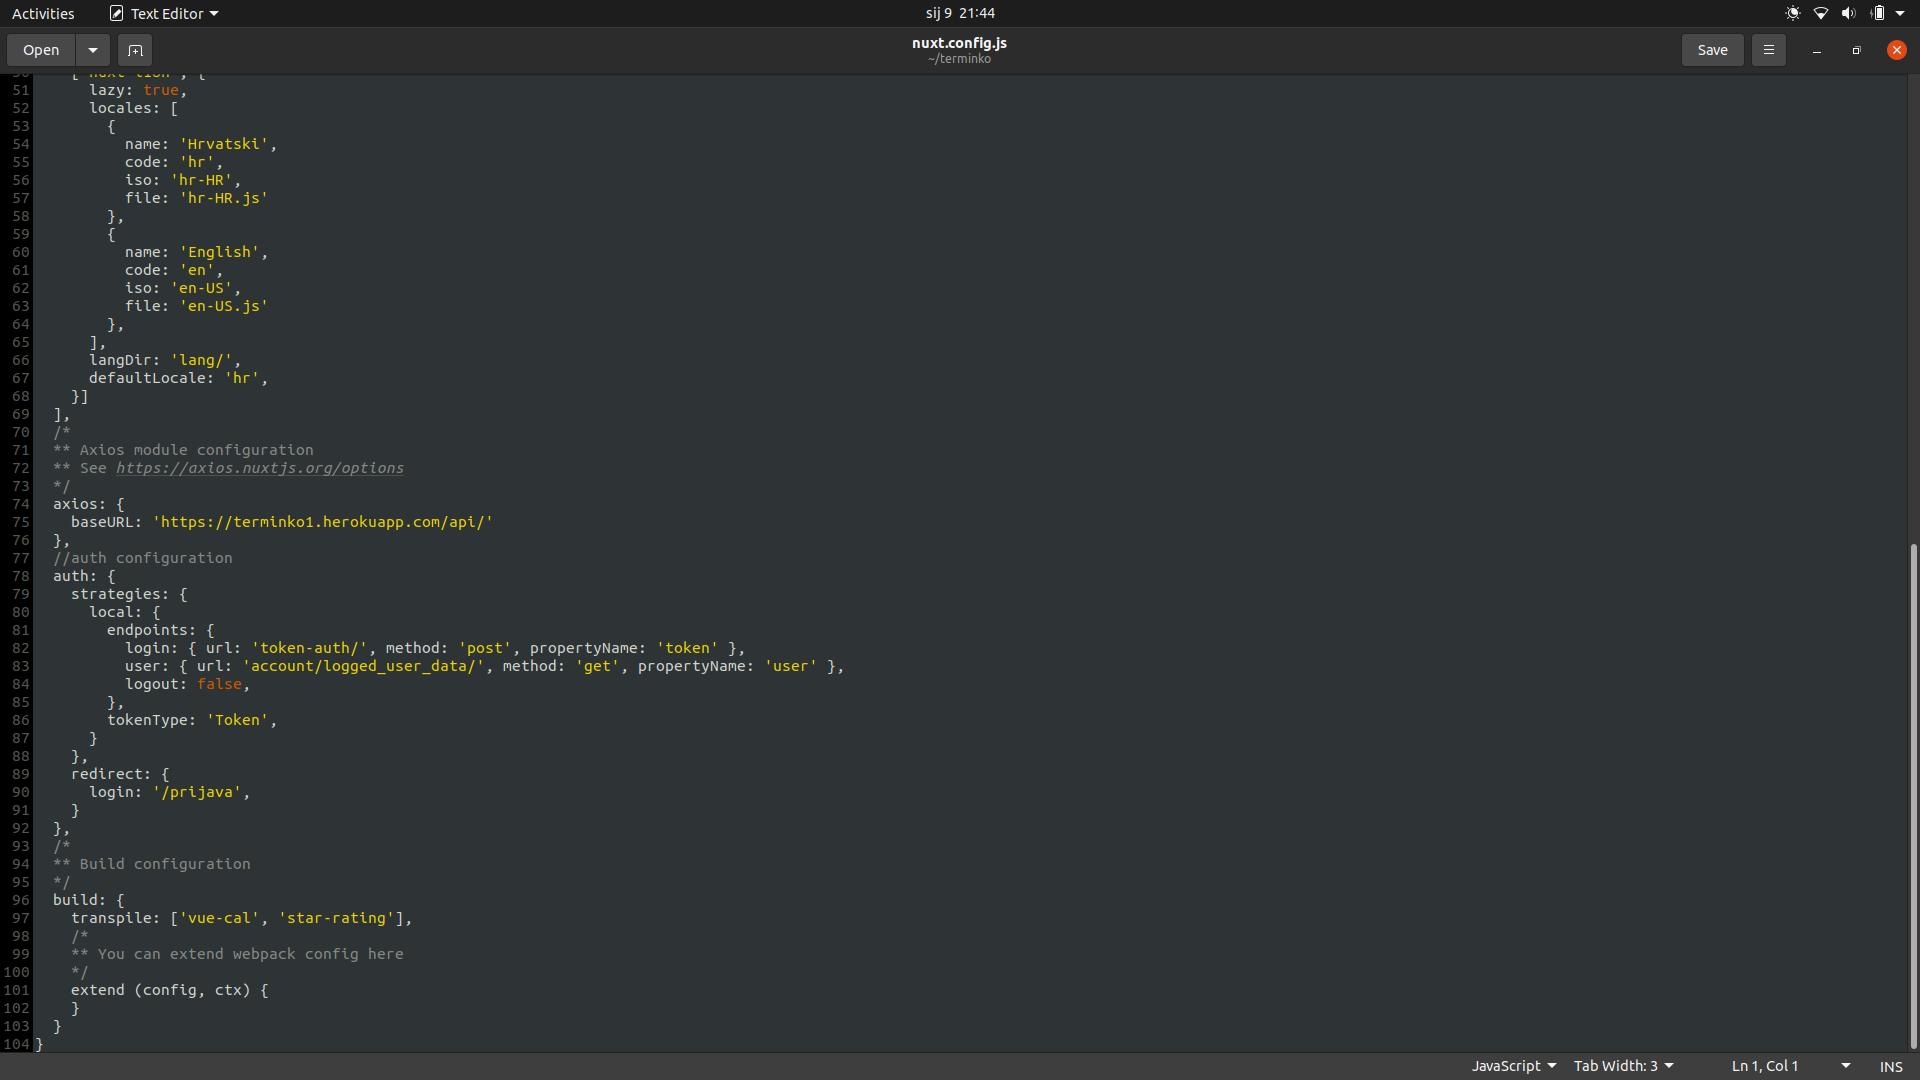
\includegraphics[scale=0.25]{slike/PromjenaFrontend.PNG}
				\caption{Promjena axios base-URL}
				\label{fig:promjene}
			\end{figure}
		
			Nakon toga, još nam je preosalo pozicionirati se u terminko mapu u terminalu, napisati naredbe git init, heroku git:remote -a terminko i git push heroku master. Nakon toga je klijentska strana bila spremna te smo krenuli s poslužiteljskom stranom.
			
			Za poslužiteljsku smo stranu napravili aplikaciju terminko1 na heroku. Na poslužiteljskoj strani nije bilo konfiguracijskih varijabli, dok smo za "buildpack" stavili heroku/python u settings odjeljku. Za razliku od fontenda, na backendu smo na heroku, u tabu resources dodali Heroku Postgres.
			
			\begin{figure}[H]
				\centering
				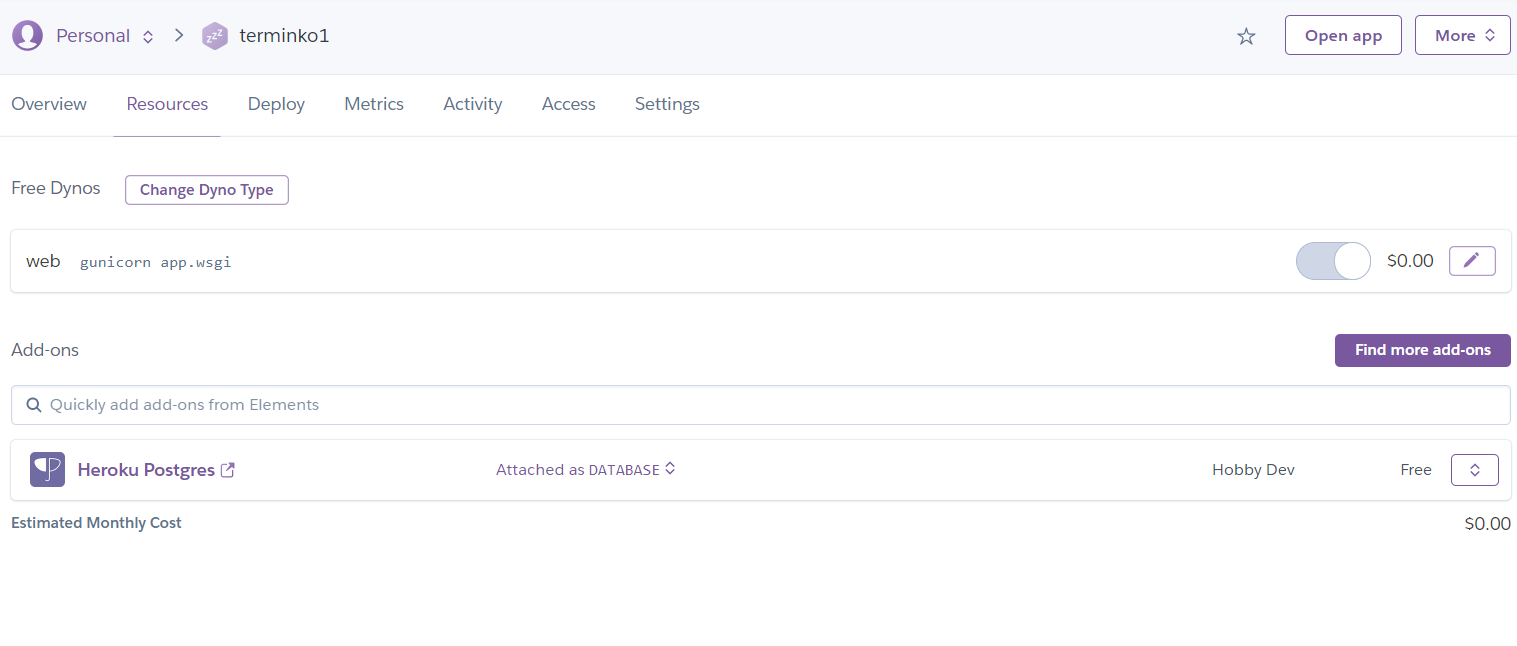
\includegraphics[scale=0.50]{slike/Postgres.PNG}
				\caption{Postavljanje Postgres baze podataka na heroku}
				\label{fig:promjene}
			\end{figure}
		
			Dakako i u mapu terminko1 morali smo dodati Procfile.
			
			\begin{figure}[H]
				\centering
				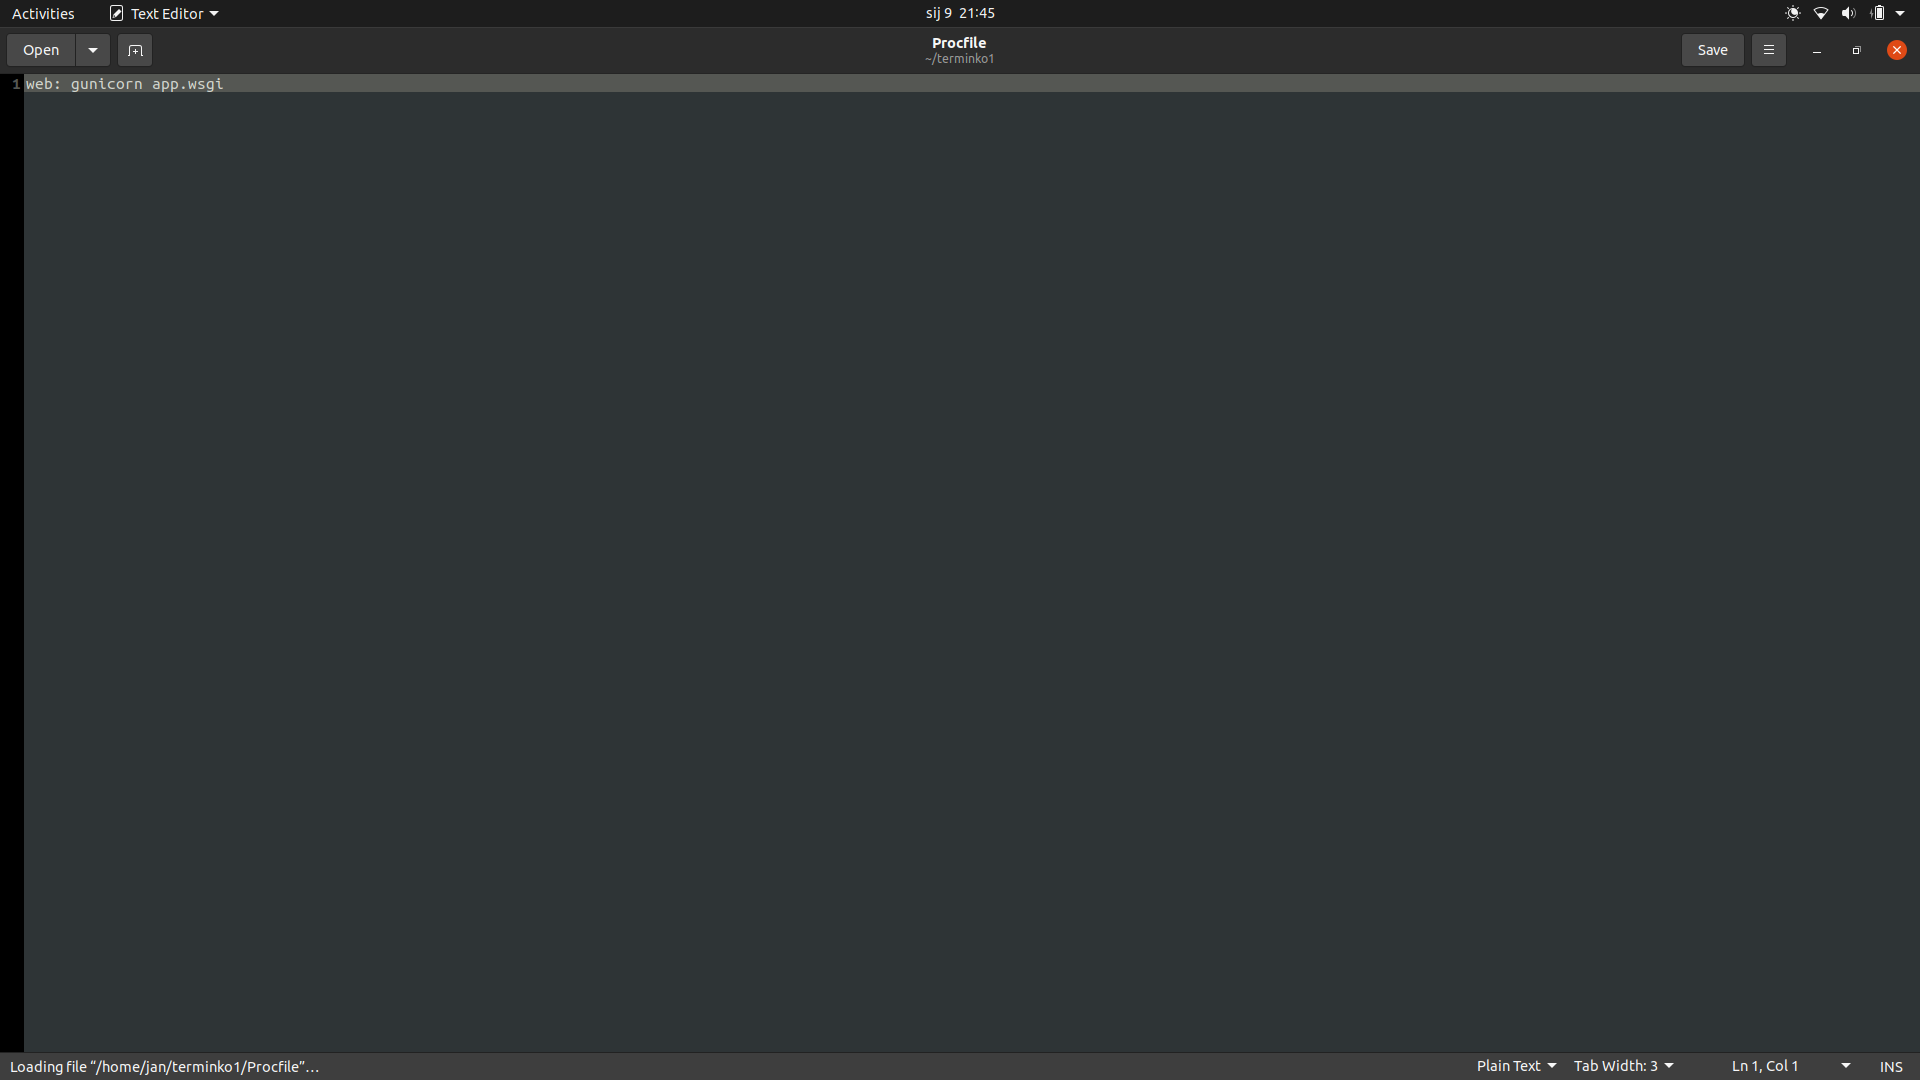
\includegraphics[scale=0.25]{slike/ProcFileBackend.PNG}
				\caption{Procfile na backendu}
				\label{fig:promjene}
			\end{figure}
		
			Nakon toga, dobili smo podatke za prijavu na postgres server koje smo stavili u settings.py datoteku na backendu. U istoj smo datoteci promjenili i CORS origin whitelist, koji označava odalke nas backend može primati zahtjeve, te allowed hosts, koji označava na kojim se poslužiteljima naš backend smije pokretati.
			
			\begin{figure}[H]
				\centering
				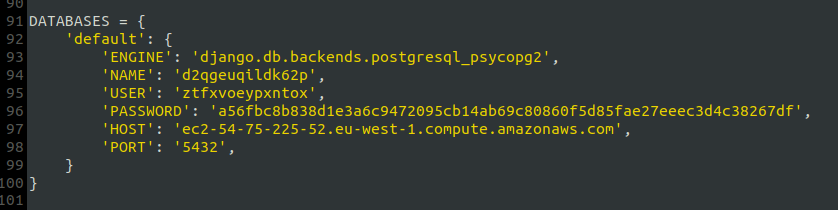
\includegraphics[scale=0.50]{slike/DatabaseData.PNG}
				\caption{Postavljanje Postgres konfiguracije u settings.py}
				\label{fig:promjene}
			\end{figure}
		
			\begin{figure}[H]
				\centering
				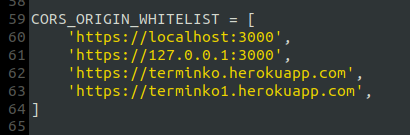
\includegraphics[scale=0.80]{slike/CorsWhitelist.PNG}
				\caption{Postavljanje cors whitelist u settings.py}
				\label{fig:promjene}
			\end{figure}
		
			\begin{figure}[H]
				\centering
				
\includegraphics[scale=0.60]{slike/AllowedHosts.PNG}
				\caption{Postavljanje allowed hosts varijable u settings.py}
				\label{fig:promjene}
			\end{figure}
		
			Nakon toga, još nam je preosalo pozicionirati se u terminko1 mapu u terminalu, napisati naredbe git init, heroku git:remote -a terminko1 i git push heroku master. Nakon toga, cijela je aplikacija bila spremna. 
			
			\begin{figure}[H]
				\centering
				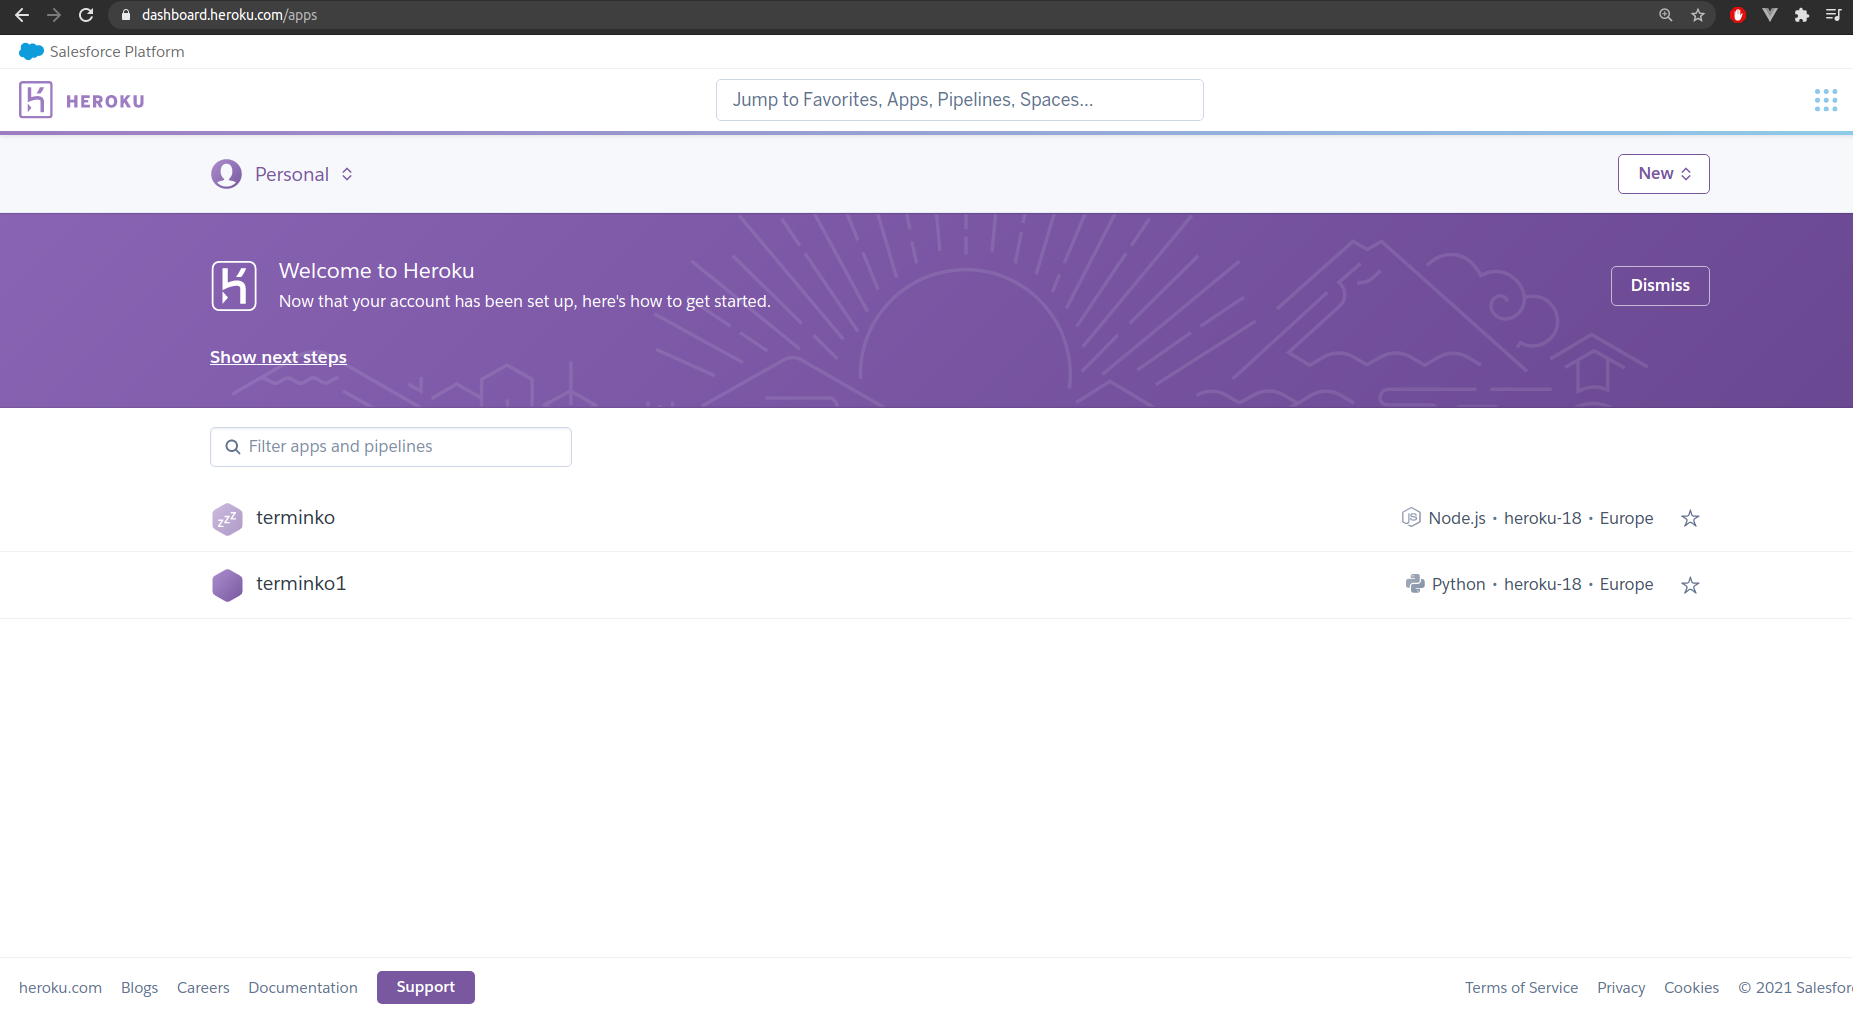
\includegraphics[scale=0.20]{slike/HerokuAplikacije.PNG}
				\caption{Prikaz stanja na heroku po završetku deploya}
				\label{fig:promjene}
			\end{figure}